\subsection{bpmorbit/bpm\_\-orbit.h File Reference}
\label{bpm__orbit_8h}\index{bpmorbit/bpm\_\-orbit.h@{bpmorbit/bpm\_\-orbit.h}}


\subsubsection{Detailed Description}
libbpm orbit generation routines 

This header contains beam oribit generation routines, so this includes also calibration scans etc... 

Definition in file {\bf bpm\_\-orbit.h}.

{\tt \#include $<$math.h$>$}\par
{\tt \#include $<$bpm/bpm\_\-defs.h$>$}\par
{\tt \#include $<$bpm/bpm\_\-units.h$>$}\par
{\tt \#include $<$bpm/bpm\_\-interface.h$>$}\par


Include dependency graph for bpm\_\-orbit.h:\nopagebreak
\begin{figure}[H]
\begin{center}
\leavevmode
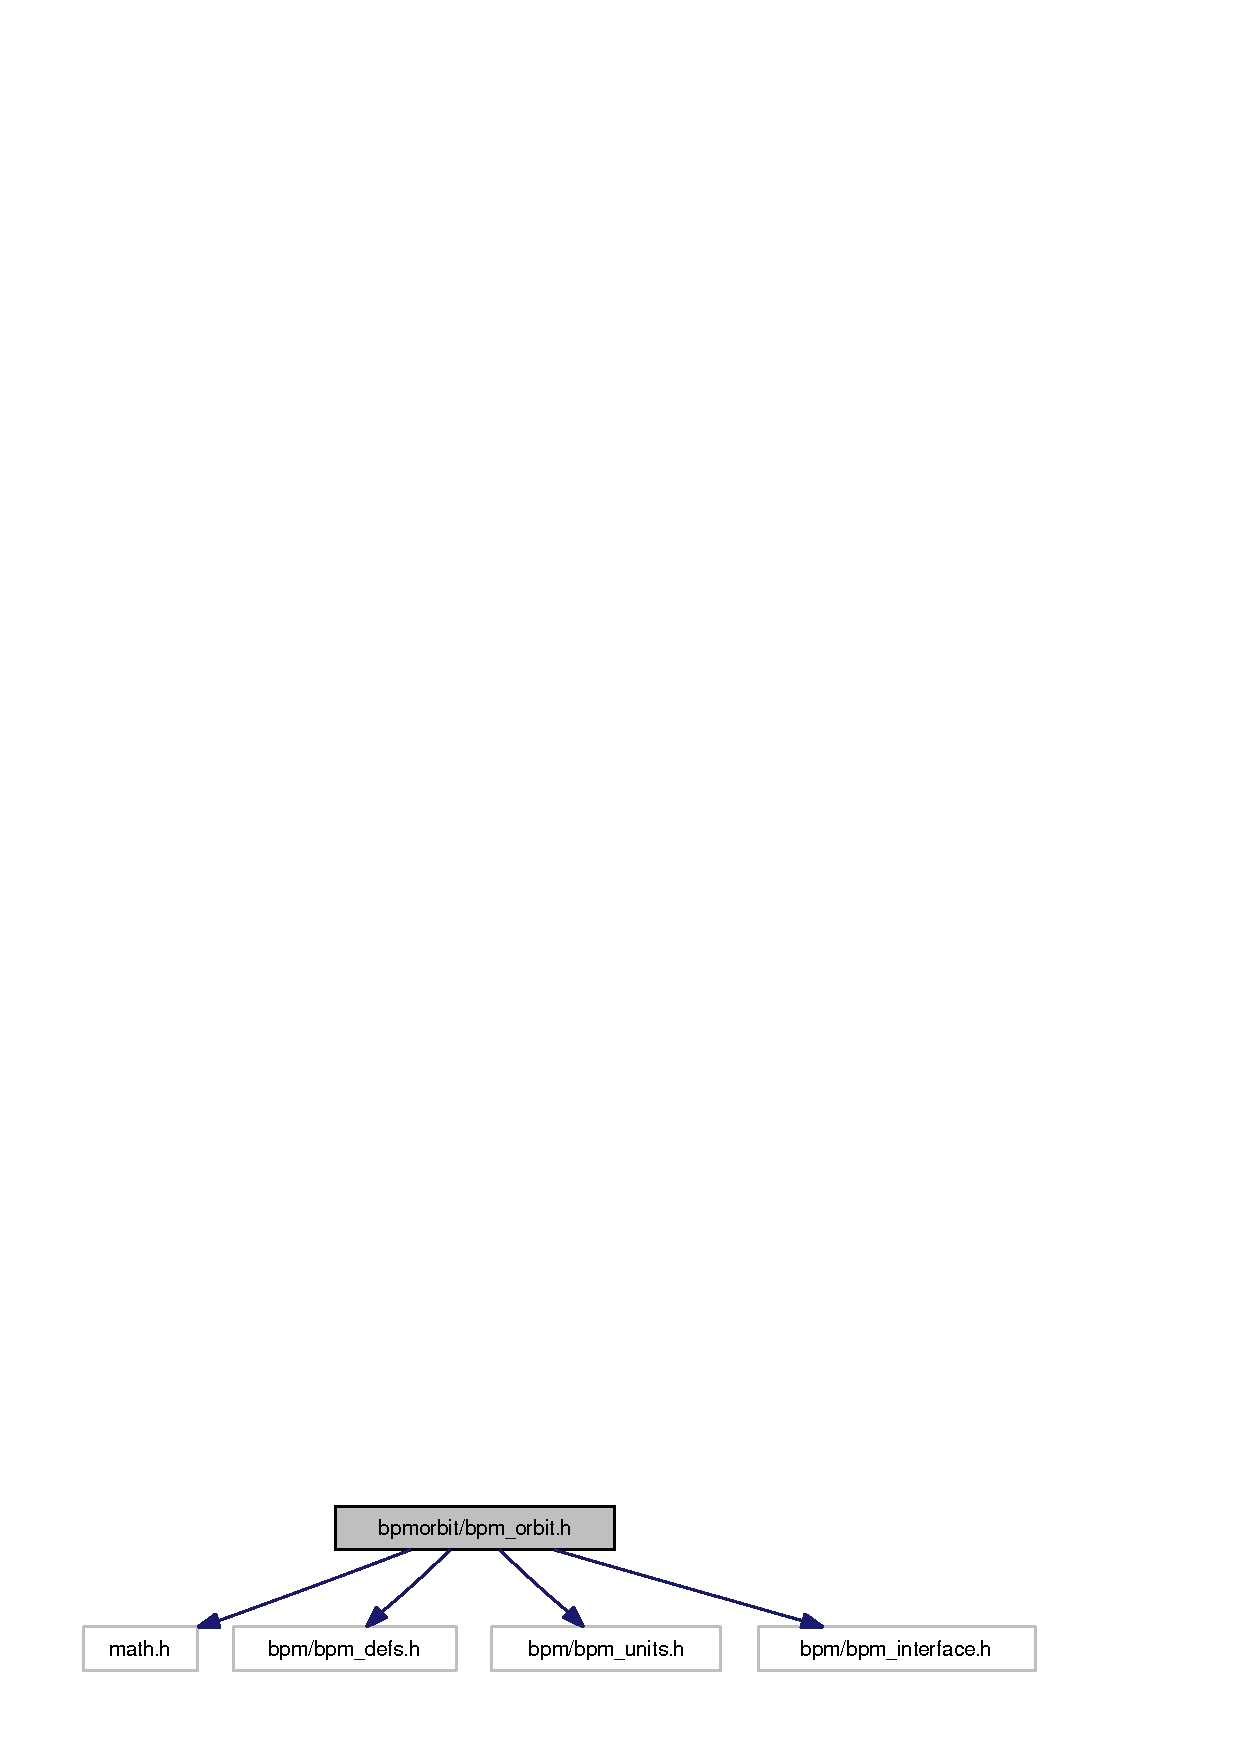
\includegraphics[width=250pt]{bpm__orbit_8h__incl}
\end{center}
\end{figure}
\subsubsection*{Data Structures}
\begin{CompactItemize}
\item 
struct {\bf v3}
\item 
struct {\bf m33}
\end{CompactItemize}
\subsubsection*{Functions}
\begin{CompactItemize}
\item 
EXTERN double {\bf get\_\-rbend} (double e, double B, double l, double p)
\item 
EXTERN double {\bf get\_\-sbend} (double e, double B, double l, double p)
\item 
EXTERN int {\bf get\_\-bpmhit} ({\bf bunchconf\_\-t} $\ast$bunch, {\bf bpmconf\_\-t} $\ast$bpm)
\item 
EXTERN int {\bf get\_\-bpmhits} ({\bf beamconf\_\-t} $\ast$beam, {\bf bpmconf\_\-t} $\ast$bpm)
\item 
void {\bf v\_\-copy} (struct {\bf v3} $\ast$v1, struct {\bf v3} $\ast$v2)
\item 
double {\bf v\_\-mag} (struct {\bf v3} $\ast$v1)
\item 
void {\bf v\_\-scale} (struct {\bf v3} $\ast$v1, double dscale)
\item 
void {\bf v\_\-norm} (struct {\bf v3} $\ast$v1)
\item 
void {\bf v\_\-matmult} (struct {\bf m33} $\ast$m1, struct {\bf v3} $\ast$v1)
\item 
void {\bf v\_\-add} (struct {\bf v3} $\ast$v1, struct {\bf v3} $\ast$v2)
\item 
void {\bf v\_\-sub} (struct {\bf v3} $\ast$v1, struct {\bf v3} $\ast$v2)
\item 
double {\bf v\_\-dot} (struct {\bf v3} $\ast$v1, struct {\bf v3} $\ast$v2)
\item 
void {\bf v\_\-cross} (struct {\bf v3} $\ast$v1, struct {\bf v3} $\ast$v2)
\item 
void {\bf v\_\-print} (struct {\bf v3} $\ast$v1)
\item 
void {\bf m\_\-rotmat} (struct {\bf m33} $\ast$m1, double alpha, double beta, double gamma)
\item 
void {\bf m\_\-matmult} (struct {\bf m33} $\ast$m, struct {\bf m33} $\ast$m1, struct {\bf m33} $\ast$m2)
\item 
void {\bf m\_\-matadd} (struct {\bf m33} $\ast$m1, struct {\bf m33} $\ast$m2)
\item 
void {\bf m\_\-print} (struct {\bf m33} $\ast$m1)
\end{CompactItemize}
